\section{Sparse matrix multiplication} \label{sec:spmm}
Sparse matrix multiplication on graphs leads to many random memory
accesses and its performance is usually limited by random memory performance
of DRAM. We perform sparse matrix multiplication in semi-external memory (SEM)
to scale to a sparse graph with billions of vertices. This strategy enables
nearly in-memory performance while achieving the scalability in proportion
to the ratio of non-zero entries to rows or columns in the sparse matrix.

\subsection{Semi-external memory}
Our definition of semi-external memory for sparse matrix multiplication is
to keep the sparse matrix on SSDs and the input dense matrix or some columns
of the input dense matrix in memory. During the computation, we stream
data in the sparse matrix from SSDs to maximize I/O throughput of the SSDs.

There are two options of keeping the output dense matrix. In applications
such as PageRank and many other graph
algorithms, dense matrices have only a few columns, so we can keep the output
dense matrix in memory for many machines. If a machine has insufficient
memory to keep the output dense matrix, we can stream the output dense matrix
to SSDs or to the subsequent computation to reduce memory consumption and
potentially I/O as well.

In some applications such as non-negative matrix factorization (Section
\ref{sec:apps}), even the input dense matrix cannot fit in memory. In this case,
we partition the input dense matrix vertically so that each partition has
complete columns of the original input dense matrix and can fit in memory.
Each vertical partition stores elements in the row-major order to increase
data locality. For each partition, we perform sparse matrix multiplication
in semi-external memory as before and stream the output matrix to SSDs.
This approach requires $\lceil \frac{D}{M} \rceil$ passes over the sparse matrix,
where $D$ is the storage size of the input dense matrix and $M$ is the memory
size.

\subsection{Sparse matrix format}
To support efficient sparse matrix multiplication in semi-external memory,
we need to use an alternative format for sparse matrices to increase CPU cache
hits and reduce the amount of data read from SSDs.
The state-of-art numeric libraries store a sparse matrix in compressed row storage
(CSR) or compressed column storage (CSC) format. However, these formats incur
many CPU cache misses in sparse matrix multiplication on real-world graphs
due to nearly random vertex connection. They also require a relatively
large storage size. For a graph with billions of edges, we have to use eight
bytes to store the row and column indices. For SEM sparse
matrix multiplication, SSDs may become the bottleneck if a sparse matrix has
a large storage size.

\begin{figure}
\centering
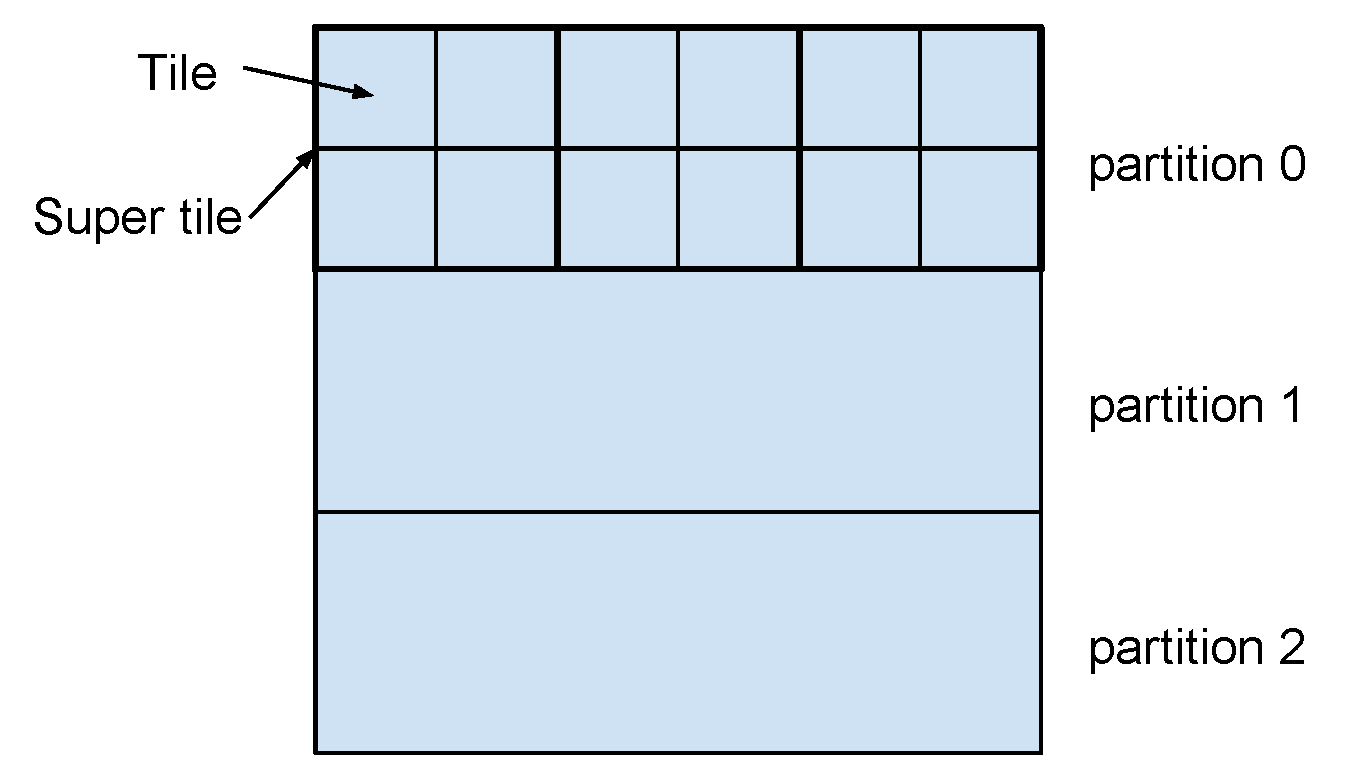
\includegraphics[scale=0.3]{./sparse_mat.pdf}
\caption{The format of a sparse matrix.}
\label{sparse_mat}
\end{figure}

To increase CPU cache hits, we deploy cache blocking \cite{Im04} and store
non-zero entries of a sparse matrix in tiles (Figure \ref{sparse_mat}).
When a tile is small, the rows from the input and output dense matrices
involved in the multiplication with the tile are always kept in the CPU cache
during the computation. The optimal tile size should fill the CPU cache
with the rows of the dense matrices involved in the multiplication with
the tile and is affected by the number of columns of the dense matrices,
specified by applications. Instead of generating a sparse matrix with
different tile sizes optimized for different numbers of columns in the dense
matrices, we use a relatively small tile size and rely on the runtime system
to optimize for different numbers of columns (in section \ref{sec:cpu}).
However, a small tile size potentially increases the storage size of the sparse
matrix. In semi-external memory, we expect that the dense matrices have
a very small number of columns in sparse matrix multiplication. Therefore, we
use the tile size of $16K \times 16K$ by default to balance the matrix storage
size and the adaptibility to different numbers of columns.

\begin{figure}
\centering
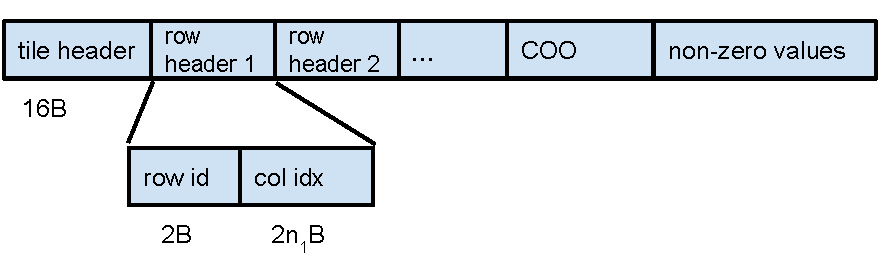
\includegraphics[scale=0.5]{./tile_format.pdf}
\caption{The storage format of a tile in a sparse matrix.}
\label{tile_format}
\end{figure}

To reduce the overall storage size of a sparse matrix, we use a compact format
to store non-zero entries in a tile. In very sparse matrices such as
many real-world graphs, many rows in a tile do not have any non-zero entries.
The CSR (CSC) format requires an entry for each row (column) in the row
(column) index. Therefore, the CSR or CSC format wastes space when storing elements
in a tile. Instead, we only keep data for rows with non-zero entries in a tile
shown in Figure \ref{tile_format} and refer to this format as SCSR (Super
Compressed Row Storage). This format maintains a row header for each non-empty
row. A row header has an identifier to indicate the row number, followed by
column indices. 
The most significant bit of the identifier is always set to 1, while the most
significant bit of a column index entry is always set to 0. As such, we can easily
distinguish a row identifier from a column index entry and determine the end
of a row. Thanks to the small size of a tile, we use two bytes to further store a row
number and a column index entry to reduce the storage size. Since the most
significant bit is used to indicate the beginning of a row, this format allows
a maximum tile size of $32K \times 32K$.

The SCSR format potentially results in many conditional jump CPU instructions
for sparse matrices with small cache blocking. As such, we hybrid SCSR and
the coordinate format (COO) to store non-zero entries in a tile to reduce
conditional jumps.
For real-world graphs, many rows in a cache tile have only one non-zero entry,
owing to the sparsity of the graphs and nearly random vertex connection.
Iterating over single-entry rows requires to test the end of a row for every
non-zero entry, which leads to many conditional jumps.
In contrast, COO is more suitable for storing these
single-entry rows. It does not increase the storage size but significantly
reduces the number of conditional jump instructions. As a result, we hybrid
SCSR and COO and store non-zero entries in the COO format behind the row headers
of SCSR (Figure \ref{tile_format}). All non-zero entries are
stored together at the end of a tile.

%We organize tiles in a sparse matrix in tile rows and maintain a matrix index
%for them. Each entry of the index stores the location of a tile row on SSDs
%to facilitate random access
%to tile rows. This is useful for parallelizing sparse matrix multiplication.
%Because a tile contains thousands of rows, the matrix index requires a very
%small storage size even for a billion-node graph. We keep the entire index
%in memory during sparse matrix multiplication.

\subsection{Dense matrices}
In many applications, dense matrices in sparse matrix multiplication are usually
tall-and-skinny matrices with millions or even billions of rows but only a small
number of columns. The number of columns is determined by applications.
In semi-external memory,
we keep the input dense matrix in memory, so its size governs memory consumption
of sparse matrix multiplication. To increase data locality in SpMM, the elements
in the dense matrices are stored in row-major order.

For a non-uniform memory architecture (NUMA), we partition the input dense matrix
horizontally and store partitions evenly across NUMA nodes. The NUMA architecture
is prevalent in today's multi-processor servers, where each processor connects
to its own memory banks. Therefore, keeping partitions evenly across all NUMA
nodes helps to fully utilize the bandwidth of memory and inter-processor links.
For horizontal partitioning, we assign multiple contiguous rows in a row
interval to a partition, which is assigned to a NUMA node. A row interval
in a partition always has $2^i$ rows for efficiently locating a row
with bit operations. The row interval size is multiple of the tile size of
a sparse matrix so that multiplication on a tile only needs to access rows
from a single row interval.

%\begin{figure}
%\centering
%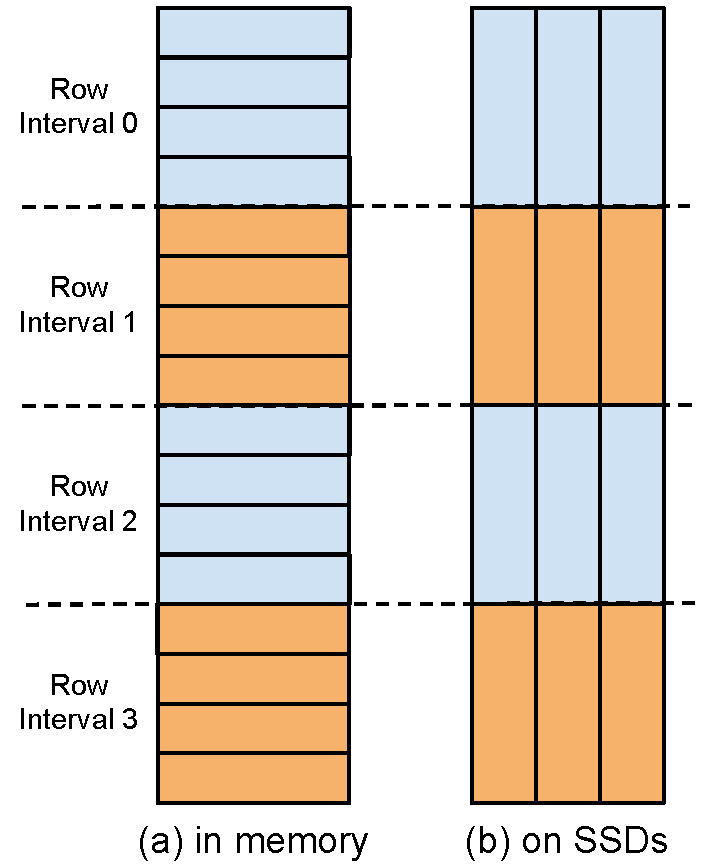
\includegraphics[scale=0.4]{./dense_matrix.pdf}
%\caption{The data layout of tall-and-skinny dense matrices. It is partitioned
%	horizontally into many row intervals.
%(a) In the input dense matrix of SpMM, row intervals are stored across NUMA nodes and
%elements are stored in the row-major order; (b) in the eigensolver, elements
%in a dense matrix inside a row interval are stored in the column-major order;
%(c) in NMF, a dense matrix is partitioned vertically first and in each partition,
%elements are stored in the row-major order.}
%\label{dense_mat}
%\end{figure}

\subsection{Runtime CPU optimizations} \label{sec:cpu}
We can perform some runtime optimizations to speed up sparse matrix
dense matrix multiplication. These runtime optimizations further reduce
CPU cache hits and allows more efficient computation and memory access.

To better utilize CPU cache, we process tiles of a partition in
\textit{super tile}s (Figure \ref{sparse_mat}). The tile size of a sparse
matrix is specified when the sparse matrix image is created and is relatively
small to handle different numbers of columns in the dense matrices.
A \textit{super tile} is composed of tiles from multiple tile rows and its
size is determined at runtime by three factors: the number of columns
in the dense matrices, the CPU cache size and the number of threads that
share the CPU cache. An optimal size for a \textit{super tile} fills
the CPU cache with the rows from the dense matrices involved in
the computation with the \textit{super tile}.

In spite of nearly random edge connection in a real-world graph,
there exists regularity \dz{explain more?} that allows vectorization to improve performance
in sparse matrix dense matrix multiplication. We multiply each non-zero entry
with the corresponding row from the input dense matrix
and add the result to the corresponding row in the output dense matrix.
These operations can be accomplished by the vector CPU instructions, such as
AVX \cite{avx} to enable more efficient memory access and computation.
The current implementation relies on GCC's auto-vectorization
to translate the C code to the vector CPU instructions by predefining the matrix
width in the code.

\subsection{I/O optimizations}
Semi-external memory sparse matrix multiplication results in sequential I/O
by streaming the sparse matrix from SSDs and potentially streaming the output
dense matrix to SSDs. For accessing fast SSDs, the overhead of operating systems
such as thread context switch and memory allocation becomes noticeable.
We need to tackle these obstacles in order to achieve the maximal I/O
throughput of fast SSDs.

The latency of a thread context switch undermines the sequential I/O throughput
of a high-speed SSD array.
%and it becomes critical to avoid thread context switch to gain I/O performance.
When a thread issues I/O and waits for I/O completion, the thread is switched
out. Once I/O is complete, the thread is rescheduled for execution but there is
latency for rescheduling. To reduce the effect of thread context switch,
an application thread issues asynchronous I/O and polls for I/O to avoid thread
context switches after completing all computation available to it.

When accessing a sparse matrix or a dense matrix from SSDs, we maintain a set of
memory buffers for I/O access to reduce the overhead of memory allocation.
We use large I/O to access matrices on SSDs to increase I/O throughput.
The operating system usually allocate a large memory buffer with \textit{mmap()}
and populates the buffer with physical pages when it is used. It is
computationally expensive to populate
large memory buffers frequently. When accessing high-throughput I/O devices,
such overhead can cause substantial performance loss. Therefore, we keep a set
of memory buffers allocated previously and reuse them for new I/O requests.
For accessing a sparse matrix, tile rows usually have differnt sizes, so we resize
a previously allocated memory buffer if it is too small for a new I/O request.

\subsection{Parallelization}
When parallelizing sparse matrix multiplication, we take into account
semi-external memory as well as the power-law distribution of non-zero entries
in each row of the sparse matrix.

We partition a sparse matrix horizontally for parallelization (Figure
\ref{sparse_mat}) to reduce thread synchronization and memory consumption.
With horizontal partitioning, a thread only needs to read tile rows assigned
to it from SSDs and processes them independently. Once the tile rows
are ready in memory, the thread multiplies the tile rows with the input
dense matrix. In addition, horizontal partitioning significantly reduce memory
consumption, which is essential for semi-external memory computation because
saved memory can be used to keep more columns in the input dense matrix in
memory to significantly reduce I/O from SSDs (as discussed in Section
\ref{sec:mem}). For example, horizontal partitioning ensures that
only the thread assigned with the tile rows need to allocate local memory buffers
for them. To reduce remote memory access in a NUMA machine, a thread needs to
store the intermediate result in a local buffer when going through all the tiles
in a partition. Horizontal partitioning also allows a small matrix index to
locate non-zero entries in the sparse matrix quickly because we only need to
locate tile rows. As such,
the matrix index is tiny even for a sparse matrix with billions of rows
and we can keep the entire matrix index in memory.

We maintain a global task queue for sparse matrix multiplication and a
thread gets one task at a time from the queue. A task may
indicates the computation on a \textit{super tile} row or a single tile row.
At the beginning of the computation, threads get larger tasks; when
the computation gets close to the end, threads get smaller tasks. This strategy
achieves good load balancing. The other benefit of maintaining a global
task queue is to maintain the global execution order, which becomes essential
when the output dense matrix needs to be written to SSDs. When a thread gets
a task, the final computation result from the task may be small. Instead of
writing the computation result immediately when it is generated, we delay
writes in order to merge
computation results from multiple threads and write them with a single I/O.
As such, we need to use the global task queue to ensure that all threads are
processing contiguous tile rows to help merge.

\subsection{The impact of the memory size on I/O in semi-external memory}
\label{sec:mem}
The memory size has significant impact on I/O in semi-external memory.
The minimum memory requirement for semi-external memory sparse matrix
multiplication is $n c + t \epsilon$, where $n$ is the number of rows
of the input dense matrix, $c$ is the element size of the dense matrix,
$t$ is the number of threads processing the sparse matrix
and $\epsilon$ is the buffer size for part of the sparse matrix and the output
dense matrix. When a machine does not have sufficient memory to keep the entire
input dense matrix in memory, we need multiple passes on the sparse matrix to
perform sparse matrix multiplication. As such, a larger memory size significantly
reduces I/O. Reducing memory consumption is essential to achieve performance
in semi-external memory because saved memory helps to keep more columns of
the input dense matrix in memory to reduce I/O.

When a machine does not have sufficient memory to keep the entire input dense
matrix, we should use the existing memory to keep as many columns in the input
dense matrix in memory as possible. Although we can use some memory to cache
part of the sparse matrix,
keeping more columns of the input dense matrix in memory saves more I/O than
using the same amount of memory to cache the sparse matrix. Assume the input
dense matrix has $n$ rows and $k$ columns. The storage size of the sparse
matrix is $E$ bytes and the memory size is $M$ bytes. We further assume
we use $M'$ bytes to keep some columns of the dense matrices in memory
($M' < M$, ${n c k} \mod {M'} \equiv 0$)
and the remaining memory ($M - M'$) to cache the sparse matrix.
The amount of data in the sparse matrix read from SSDs is
\begin{equation*}
IO_{in} = \frac{n c k}{M'} [E - (M - M')]
\end{equation*}
Because $E > M$ in semi-external memory, we can minimize $IO_{in}$ by maximizing $M'$.
Therefore, using memory for the input dense matrix always results in a smaller
amount of I/O than using memory for caching the sparse matrix.

As the number of columns from the input dense matrix kept in memory increases,
the bottleneck of the system
may switch. When we keep only one column of the input dense matrix in memory,
the system is usually I/O bound; when we can keep more columns of the dense matrix
in memory, the system will become CPU bound. Once sparse matrix multiplication
becomes CPU bound, the I/O complexity does not affect its performance.
%and the additional memory does not improve
%the performance of sparse matrix multiplication further.

%Our strategy results in the minimum amount of data written to SSDs. When the output
%dense matrix cannot fit in memory, the maximum write is $N k$ for a square
%sparse matrix.
%In other words, the output matrix only needs to be written to SSDs at most once.
%The additional memory in the system can be used to buffer part of the output
%dense matrix to reduce the amount of data written to SSDs. Streaming the output
%matrix directly to the subsequent matrix computation can also reduce data written
%to SSDs.

\subsection{I/O complexity}
The semi-external memory (SEM) solution for sparse matrix multiplication leads
to no more I/O than the external-memory (EM) solution for many real-world graphs.

When a machine has sufficient memory to keep the entire input dense matrix
in memory, the SEM solution only needs to read the sparse matrix and the input
dense matrix once and write the output dense matrix once. This results in
a minimum amount of I/O. As such, the SEM solution does not cause more I/O
than any EM solutions.

When a machine has insufficient memory to keep the input dense matrix, the SEM
solution still leads to less I/O than the EM solution when $E < n c k t$.
In the analysis, we assume a square sparse matrix. The same analysis applies
to a rectangular sparse matrix as well.
In this case, the SEM solution scans the sparse matrix multiple times.
\begin{equation*}
read_{SEM} = \frac{n c k}{M} E + n c k
\end{equation*}
To minimize writes, the EM solution
scans the sparse matrix once but reads the input dense matrix multiple times.
Due to near vertex connection in real-world graphs, the EM solution needs to
read the entire input dense matrices each time. In the parallel setting,
the EM solution requires each thread to keep local memory buffers for portions
of the input and output dense matrices. Assume the EM solution keeps $j$ rows
from the input dense matrix and $i$ rows from the output dense matrix in memory
in each thread.
\begin{equation*}
(i c k + j c k) t = M => i < \frac{M}{c k t}
\end{equation*}
\begin{equation*}
read_{EM} = \frac{n}{i} n c k + E =>  read_{EM} > \frac{n^2 c^2 k^2 t}{M} + E
\end{equation*}
When $n c k < E < n c k t$, $read_{EM} > read_{SEM}$.
When $E \leq n c k$, $read_{EM} > read_{SEM}$ for any $t \geq 2$.

As such, the SEM solution in practice causes less I/O in many natural graphs.
For the natural graphs that we have seen, such as Twitter \cite{twitter},
the Page graph \cite{web_graph} and Friendster \cite{friendster}, the number
of edges is of $10-100 \times$ the number of vertices. Essentially,
natural graphs have sparse edge matrices. We target multi-core machines with
10s to 100s of threads. For most of our applications, $k$ is of size 1-30.
For very small $k$, the SEM
solution can keep the entire input dense matrix in memory and leads to minimum
I/O. For a relatively larger $k$, $E < n c k t$ holds
for most of natural graphs. Therefore, the SEM solution usually performs less
I/O than EM.

\section{Applications} \label{sec:apps}
We apply sparse matrix multiplication to three important applications widely
used in data mining and machine learning: PageRank \cite{pagerank},
eigensolver \cite{anasazi} and non-negative matrix factorization \cite{nmf}.
Each application demonstrates a different strategy of using memory for sparse
matrix multiplication.

\subsection{PageRank} \label{sec:pagerank}
PageRank is an algorithm to rank the Web pages by using hyperlinks between Web
pages. It was first used by Google and is identified as one of the top 10 data
mining algorithms \cite{top10}. PageRank is a representative of a set of graph
algorithms that can be expressed with sparse matrix multiplication or generalized
sparse matrix multiplication. Other important examples are label propagation
\cite{label_prop} and belief propagation \cite{Yedidia03}. The algorithm runs
iteratively and its update rule for each Web pages in an iteration is
\begin{equation*}
PR(u) = \frac{1-d}{N} + d \sum\limits_{v \in B(u)} \frac{PR(v)}{L(v)}
\end{equation*}
where $B(u)$ denotes the neighbor list of vertex $u$ and $L(v)$ denotes
the out-degree of vertex $v$. We implement the PageRank algorithm with sparse
matrix multiplication (Figure \ref{code:pagerank}).


\begin{figure}
\centering
%\begin{minted}[mathescape, fontsize=\scriptsize,]{r}
\begin{lstlisting}
while (L1 >= epsilon && niters < max.niters) {
	pr2 <- d/N+(1-d)*(A %*% (pr1/out.deg))
	L1 <- sum(abs(pr1-pr2))
	pr1 <- pr2
	niters <- niters + 1
}
\end{lstlisting}
%\end{minted}
\caption{The implementation of PageRank with SpMM.}
\label{code:pagerank}
\end{figure}

%Based on the memory size, we can place different data in memory to reduce I/O.
%When the memory can only fit a single vector, each iteration needs
%to write a vector to SSDs and read two vectors (the result from
%the previous iteration and the degree vector) and the sparse matrix
%from SSDs. When the memory can fit two vectors, the output vector can be kept
%in memory, so each iteration needs to read the sparse matrix and the degree vector
%and does not write any data to SSDs. As more memory can be used, we can
%further keep the degree vector and even cache part of the sparse matrix.

\subsection{Eigensolver}
An eigensolver is another commonly used application that requires sparse matrix
multiplication. Many algorithms \cite{Lanczos, IRLM, krylovschur} and frameworks
\cite{arpack, anasazi, slepc} have been developed to solve a large eigenvalue
problem.

We take advantage of the Anasazi eigensolver framework \cite{anasazi} and
replace its original matrix operations with our SEM sparse
matrix multiplication and external-memory dense matrix operations. To compute
eigenvalues of a $n \times n$ matrix, many eigenvalue algorithms for a large
sparse matrix require to construct a vector subspace with a sequence of
sparse matrix multiplication and each vector in the subspace has the length of $n$.
Due to the sparsity of many real-world graphs such as social networks,
the vector subspace requires substantial storage size and we keep
some of the vectors in the subspace on SSDs. In addition to sparse matrix
multiplication, eigensolvers perform some dense matrix operations on the subspace.
For example, eigensolvers need to orthogonalize the vectors in the subspace with
dense matrix multiplication. The Anasazi eigensolvers have block extension to
update multiple
vectors in the subspace simultaneously and thus require sparse matrix dense
matrix multiplication. The most efficient Anasazi eigensolver on sparse graphs
is the KrylovSchur eigensolver \cite{krylovschur}, which updates a small number
of vectors (1-4) in the subspace simultaneously. Zheng et al.
\cite{flasheigen} provides the details of extending the Anasazi eigensolver
with external-memory matrix operations.

%The choice of data placement for an eigensolver is a little different from
%PageRank. If a machine has a small amount of memory, the memory should be
%used to keep the input dense matrix. If a machine has more memory, we should
%use it to buffer the output dense matrix. The dense matrices involved in
%sparse matrix multiplication have a small number of columns in
%the KrylovSchur eigensolver and usually can fit in memory. 
%Additional memory should be used to buffer the vectors in the subspace
%to reduce I/O for dense matrix operations.

\subsection{Non-negative matrix factorization}
Non-negative matrix factorization (NMF) \cite{nmf} is to find two non-negative
low-rank matrices $W$ and $H$ to approximate a matrix $A \approx WH$. NMF is
typically used to find factorization on sparse matrices. NMF has many applications
in machine learning
and data mining. A well-known example is collaborative filtering \cite{cf} in
recommender systems. NMF is also applied to graphs, for example, to find communities
\cite{yang13, wang11}.

Many algorithms are designed to solve NMF and here we describe an algorithm
\cite{nmf} that requires a sequence of sparse matrix multiplication.
The algorithm uses multiplicative update rules and updates matrices $W$ and $H$
alternately. In each iteration, the algorithm first fixes $W$ to update $H$
and then fixes $H$ to update $W$.
\begin{equation*}
H_{a\mu} \leftarrow H_{a\mu} \frac{{(W^TA)}_{a\mu}}{{(W^TWH)}_{a\mu}},
W_{ia} \leftarrow W_{ia} \frac{{(AH^T)}_{ia}}{{(WHH^T)}_{ia}}
\end{equation*}

We apply SEM sparse matrix multiplication to NMF differently
based on the memory size and the number of columns in $W$ and $H$. Due to
the sparsity of a graph, it is possible that the non-negative matrices $W$ and
$H$ may require the storage as large as the sparse matrix and can no longer fit in
memory. Therefore, we need to partition $W$ and $H$ vertically and run multiple
sparse matrix multiplications to compute $W^TA$ and $AH^T$, if the memory is not
large enough to keep $W$ and $H$.

%The choices of data placement for NMF are
%shown as follows. If memory is small, all memory should be used to keep as many
%columns in the input dense matrix as possible to reduce I/O. The original sparse
%matrix multiplication is broken into multiple multiplications. We stream the output
%dense matrices to SSDs and construct some of the input dense matrices for the next
%sparse matrix multiplications in memory to reduce the latency of loading
%the input dense matrix to memory. The additional memory in a machine can be used
%to buffer the output dense matrix of sparse matrix multiplication.
